\chapter{CAD Model}\label{cp:cad}

Our initial \acrfull{cad} model is shown in \autoref{fig:cad_w_dimensions} and \autoref{fig:3d_model}.

\begin{figure}[htpb]
    \centering
    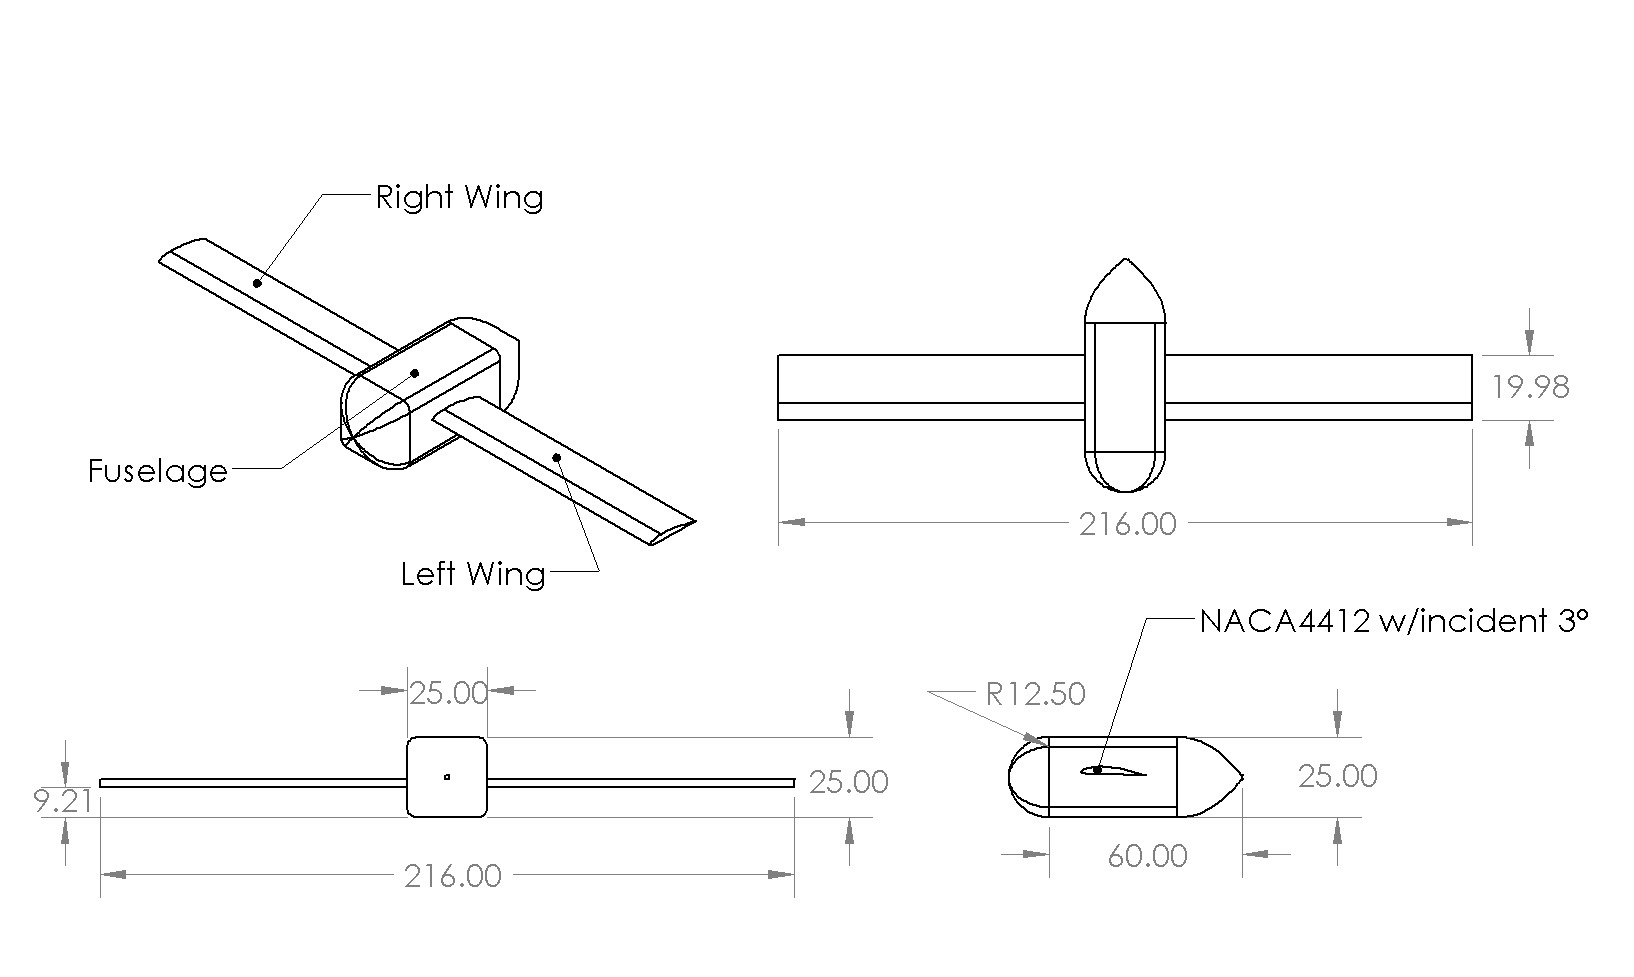
\includegraphics[width=\linewidth]{Figures/FuselageAirfoilAssemDraw.JPG}
    \caption[\acrshort{cad} model with dimensions]{The preliminary \acrshort{cad} model used for aerodynamic analysis with dimensions. All unlabeled dimensions are in units of \unit{\centi\meter}.}
    \label{fig:cad_w_dimensions}
\end{figure}

\begin{figure}[htpb]
    \centering
    \begin{subfigure}{0.5\textwidth}
        \centering
        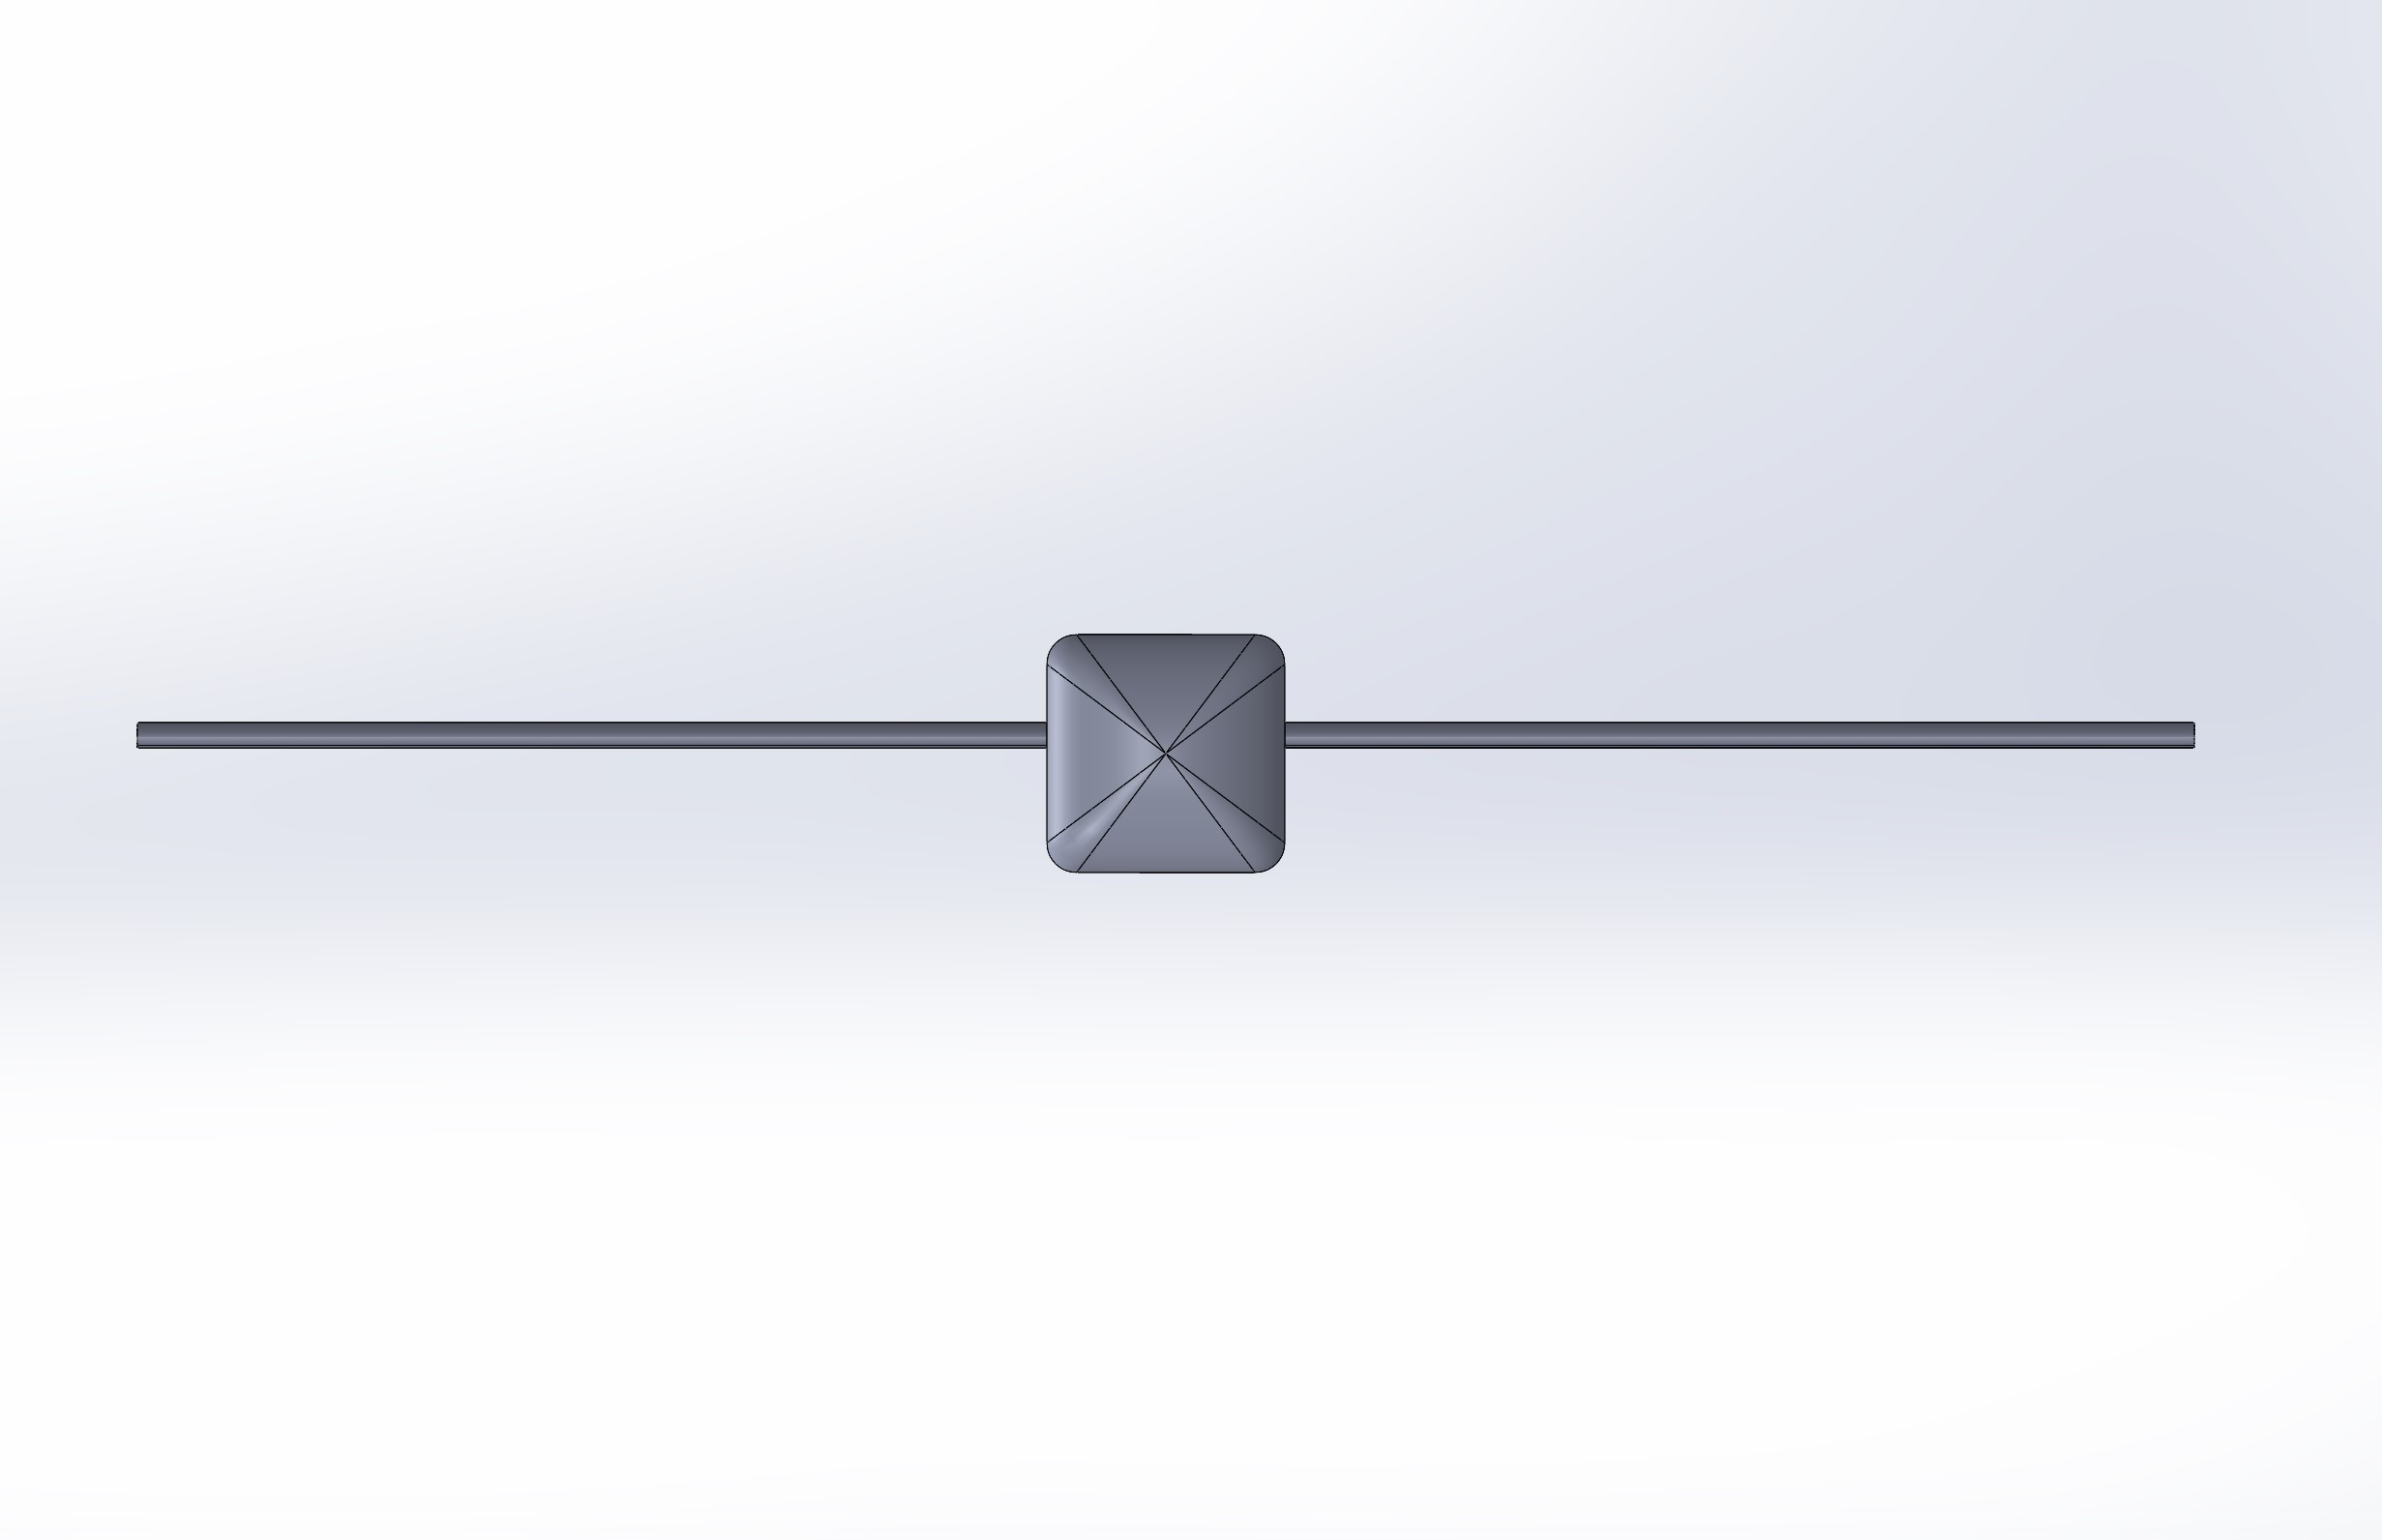
\includegraphics[width=\textwidth]{Figures/Frontview9_29.jpg}
        \caption{3D aircraft model (front view).}
        \label{fig:3d_front}
    \end{subfigure}\\
    \begin{subfigure}{0.5\textwidth}
        \centering
        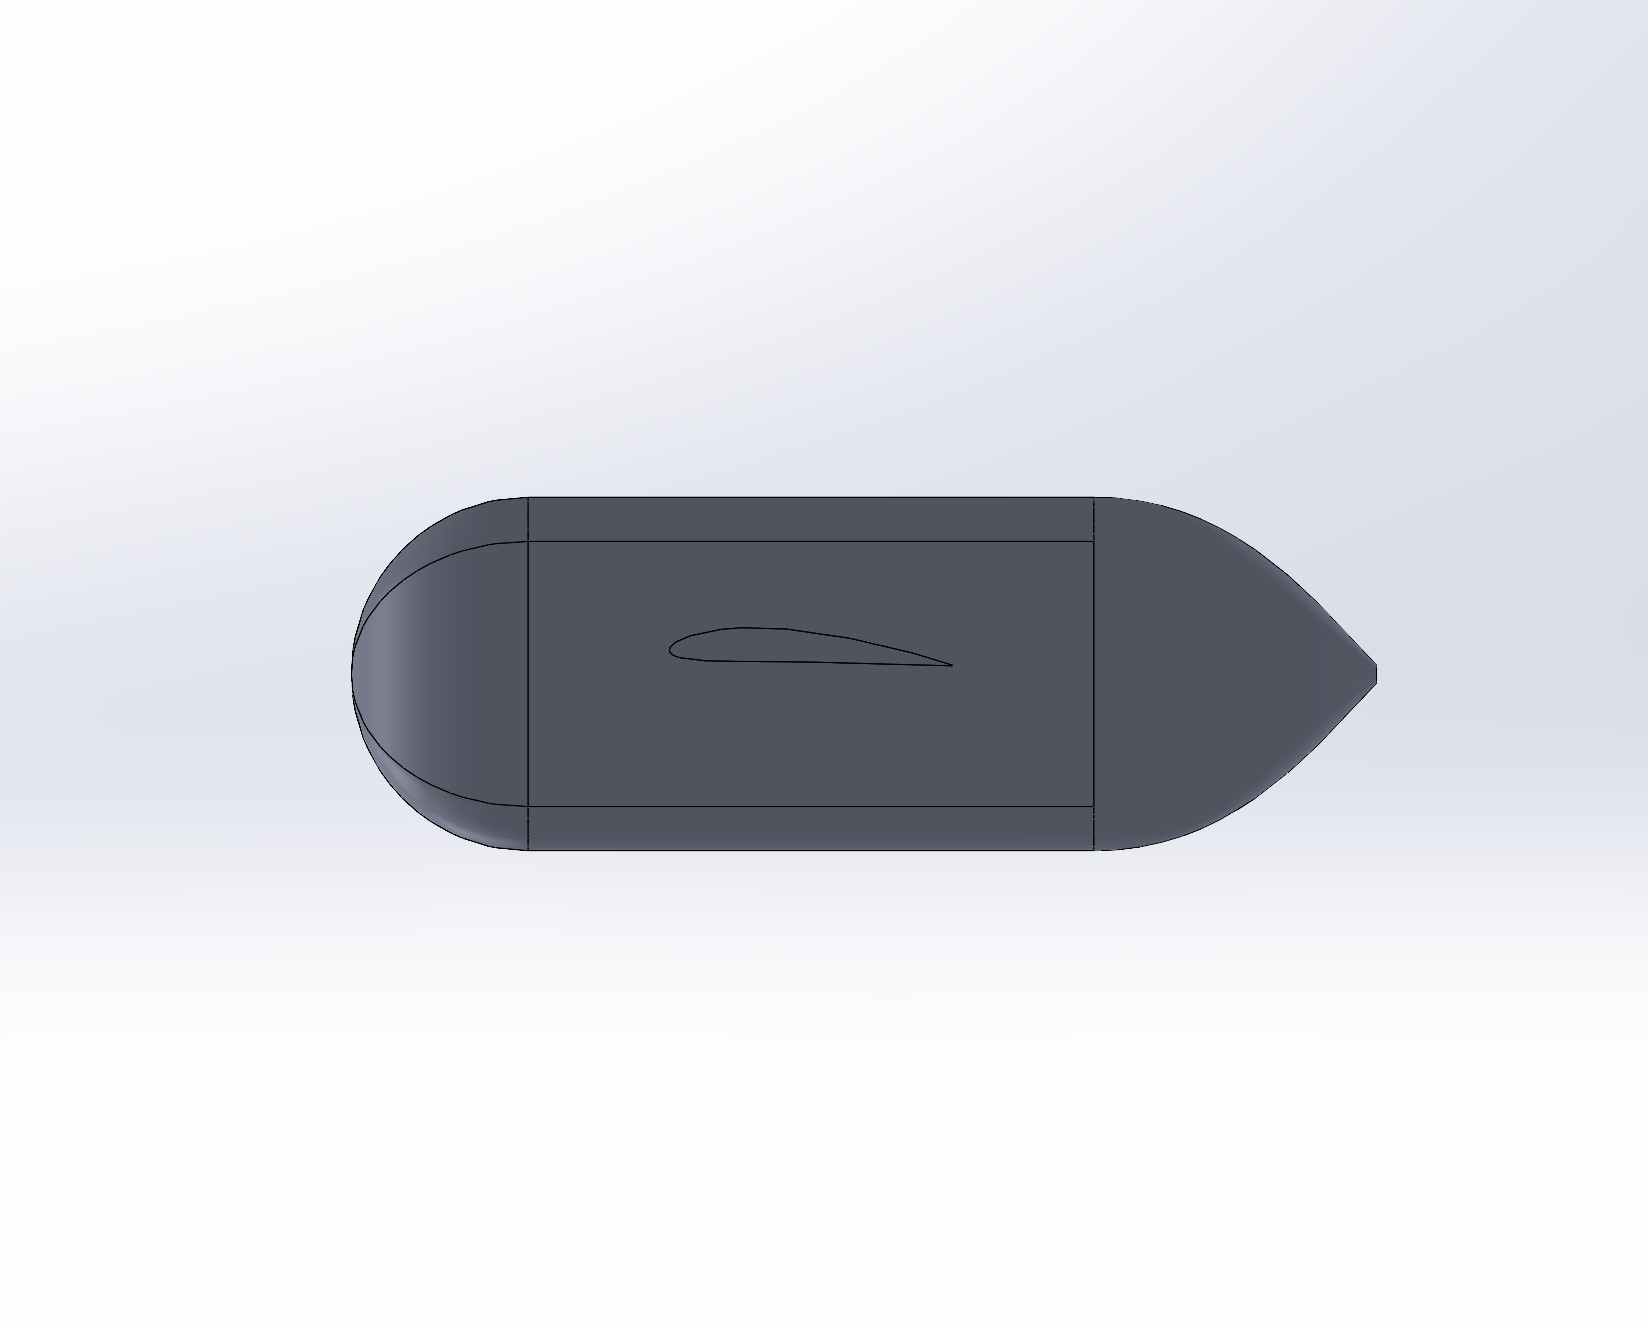
\includegraphics[width=\textwidth]{Figures/SideView9_29.jpg}
        \caption{3D aircraft model (side view).}
        \label{fig:3d_side}
    \end{subfigure} \\
    \begin{subfigure}{0.5\textwidth}
        \centering
        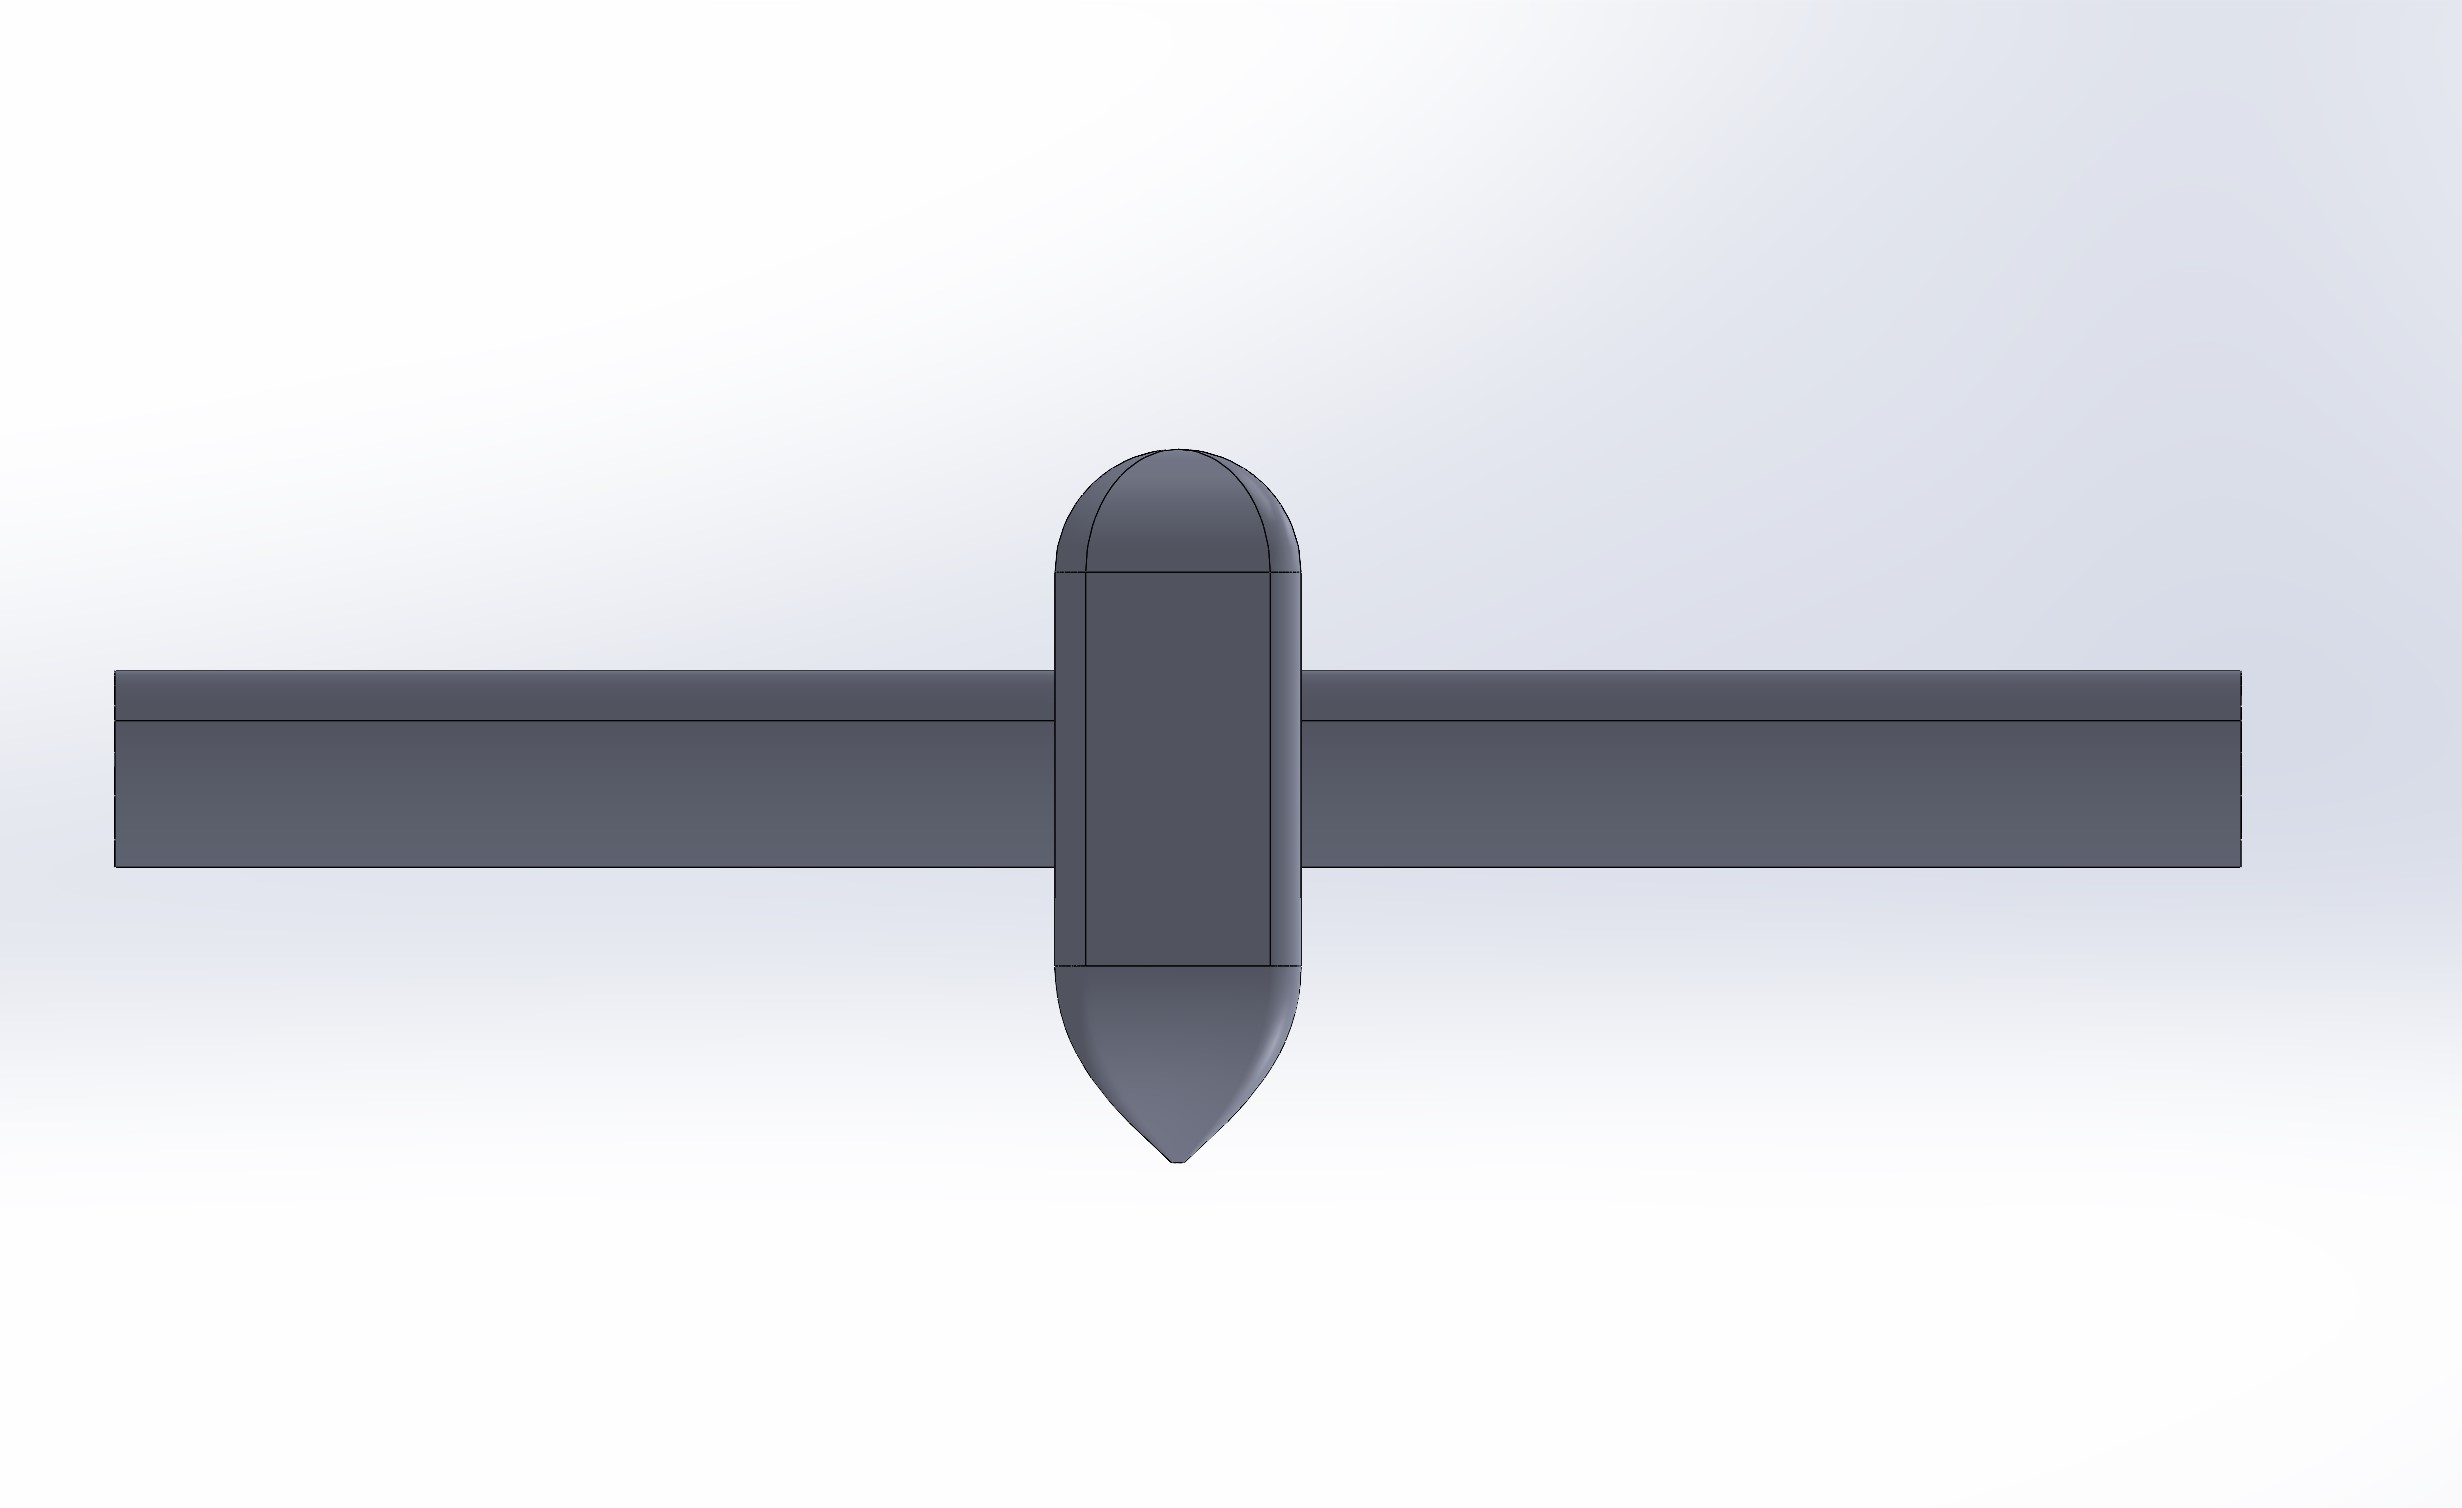
\includegraphics[width=\textwidth]{Figures/TopView9_29.jpg}
        \caption{3D aircraft model (top view).}
        \label{fig:3d_top}
    \end{subfigure}\\
    \begin{subfigure}{0.5\textwidth}
        \centering
        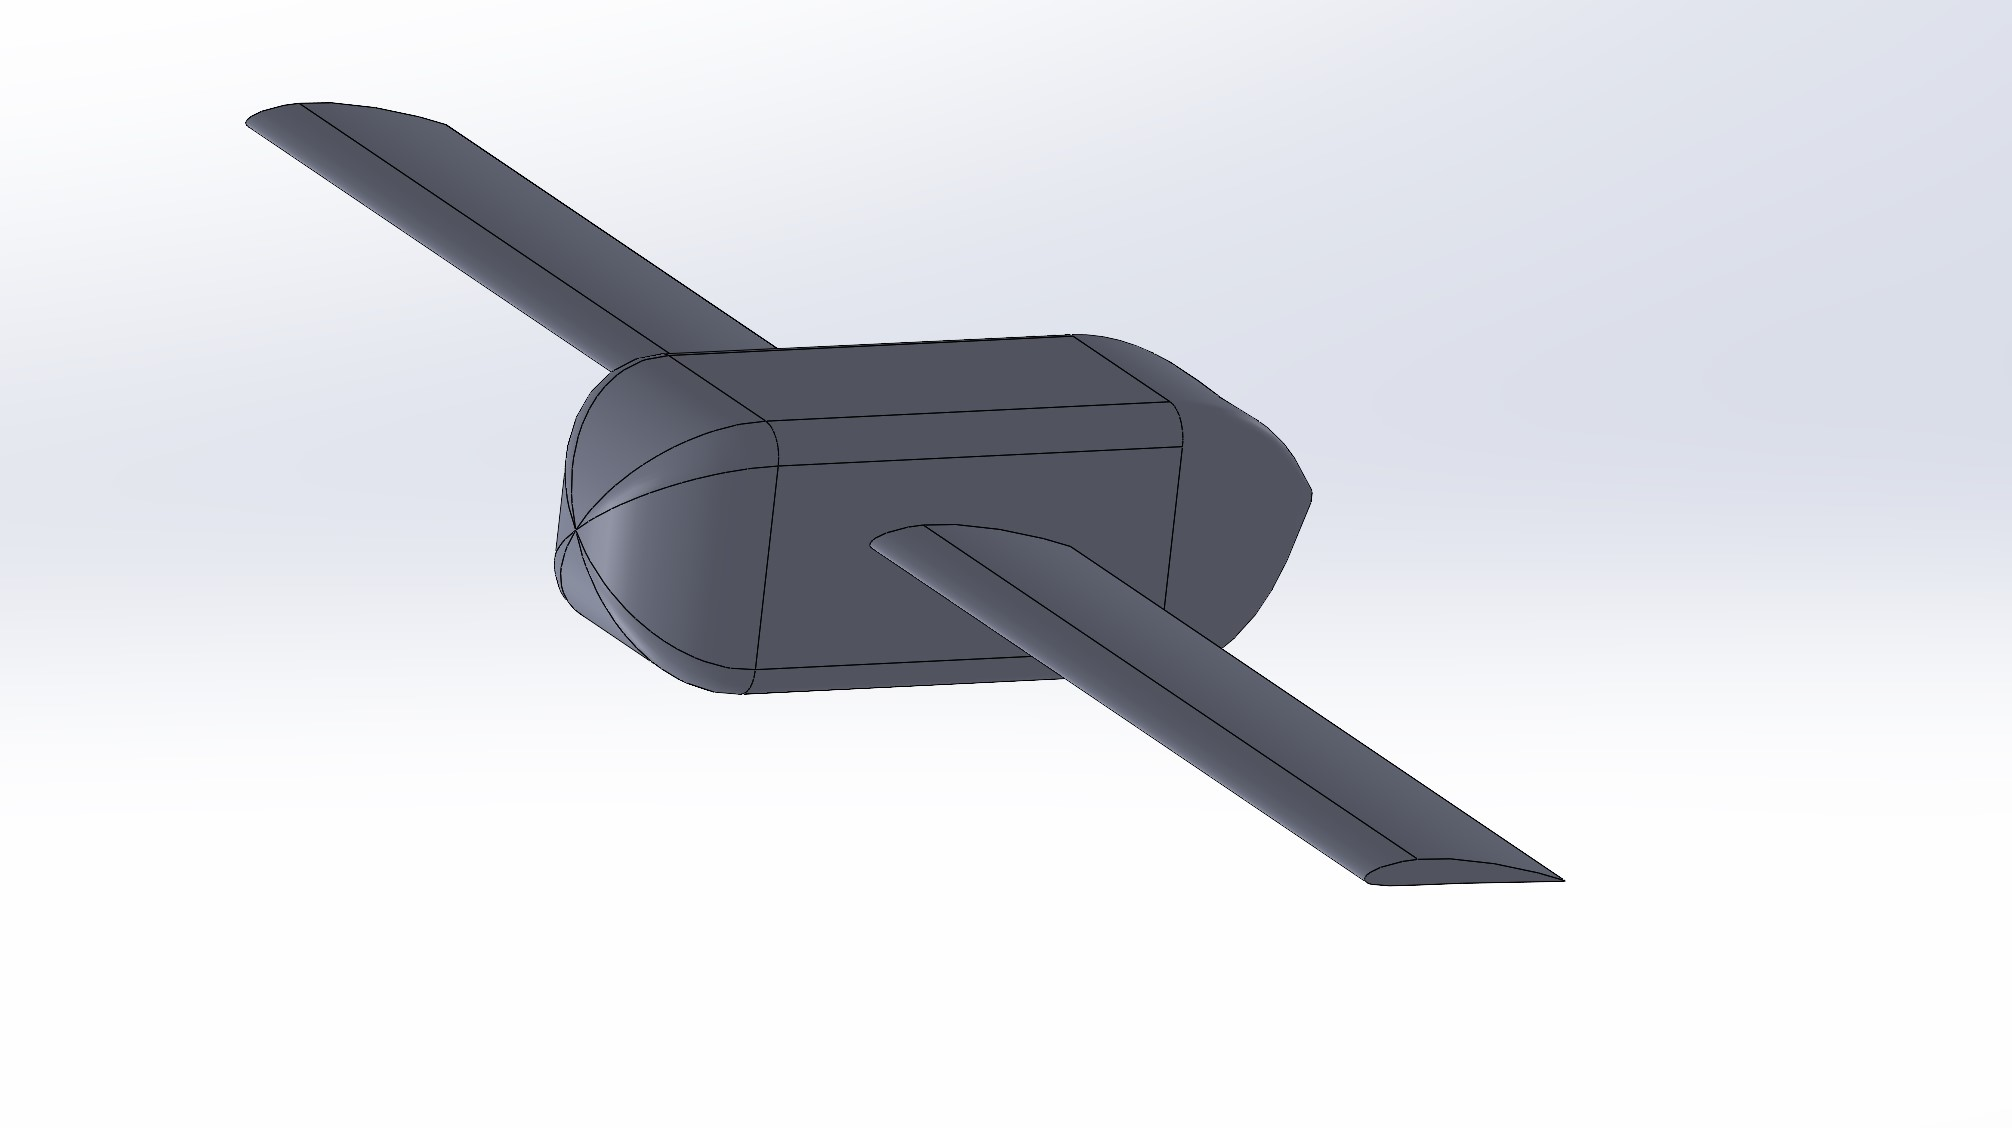
\includegraphics[width=\textwidth]{Figures/IsoView9_29.jpg}
        \caption{3D aircraft model (isometric view).}
        \label{fig:3d_isometric}
    \end{subfigure}
    \caption[3D model of the aircraft]{Different views of the SolidWorks model.}
    \label{fig:3d_model}
\end{figure}
